%!TEX root = ../Thesis.tex

\section{Controller Logic} % (fold)
\label{sec:controller_logic}
The autonomous landing system developed in this work is just a piece of FFI's autonomous UAV platform. All control systems and sensor modules are controlled by the \gls{HAL} module, that takes the high level decisions and delegates task to underlaying modules. For instance, during a search and rescue mission HAL takes the decision of when the UAV have to change battery. HAL then requests autonomous landing on to the battery exchange robot mounted on a moving vehicle. The autonomous landing system then starts performing its landing sequence. At any time during the landing operation, HAL may reschedule and disable the landing. 
For safety reasons, the velocity set-point generated by the landing controller, and all other control modules are sent to a safety node. The safety node checks the velocity set-point and restricts it if necessary before it sends the velocity command to the UAV flight controller. The safety module do also switch to manual control as soon as someone uses the remote control. 

The set-point and HAL communication-flow described in this section are illustrated in Figure~\ref{fig:sp_flow}
\begin{figure}[ht]
	\begin{center}
		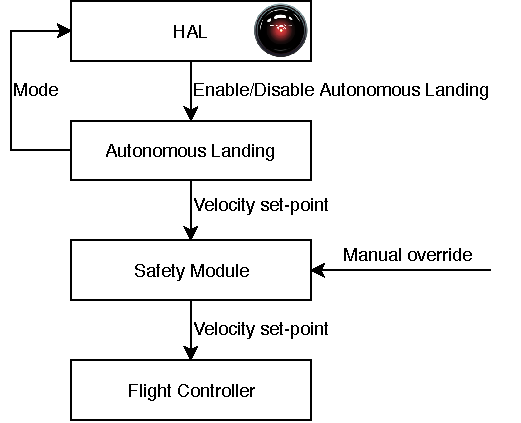
\includegraphics[scale=1.0]{img/sp_flow}
        \caption{Velocity set-point and HAL communication flow chart}
        \label{fig:sp_flow}
	\end{center}
\end{figure}

\subsection{State machine} % (fold)
\label{sub:state_machine}
This section takes a close look at the state machine used to implement the autonomous landing system. The state machine in this section returns position set-point and a controller gain to be fed in to a target tracking controller. Two target tracking controllers are derived in closer details in section~\ref{sec:guidance_methods}. The state machine do also return a boolean output to the flight controller to trigger a force land command. This command tels the flight controller to ignore the velocity set-point and just go straight down and turn of its propellers when it touches the ground.

\begin{figure}[ht]
	\begin{center}
		\def\svgwidth{0.70\columnwidth}%{0.70}
		\import{img/}{Landing_modes.pdf_tex}
        \caption{State machine states visualized for a UAV landing on a vehicle}
        \label{fig:landing_modes}
	\end{center}
\end{figure}

The state machine is built up with seven states. Stop, Intercept, Hover, Lower, Gain adjust, Final stage and Land. Figure~\ref{fig:landing_modes} gives a graphical illustration of the different states. The state stop, is only activated when autonomous landing is disabled and will the return zero as velocity output. The intercept state has the purpose of bringing the UAV to the hover point located at a fixed distance above the landing pad. In hover mode, the UAV will stay in this hover point fixed above the landing pad while the position state estimator improves its estimates. This hover point is selected at a certain height that ensures the landing pad to be fixed within the camera field of view. The state machine will stay in this state until the covariance of the position estimate reaches an acceptable level. The lower state lowers the UAV towards the landing pad at a given descent velocity. When the UAV reaches a certain height, the state machine enters the gain adjust state. This state adjusts the controller gain to a more aggressive gain to ensure a more precise position control. At the final stage state, the descent velocity is reduced to get an even more precise position control. And finally, the land states triggers the force land command to the flight controller, which brings the UAV all the way down to the landing pad and disarms the motors. Algorithm~\ref{alg:state_machine_output} lists a pseudo code to summarize the state machine outputs in the different states.

\begin{algorithm}
\caption{State machine output}\label{alg:state_machine_output}
	\begin{algorithmic}[1]
		\State $\Delta t=getCurrentTime()-t_0$
		\If{$state=stop$}
			\State $Stop$
		\ElsIf{$state = intercept\: \mathbf{or} \: hover$}
			\State $gain \gets gain_{1}$
			\State $pos_{sp} \gets hooverHeight$
		\ElsIf{$state = lower$}
			\State $gain \gets gain_{1}$
			\State $pos_{sp} \gets pos_{sp}-decentVel_u \Delta t$
		\ElsIf{$state = gainAdjust$}
			\State $gain \gets gain_{2}$
			\State $pos_{sp} \gets pos_{sp}-decentVel_u \Delta t$
		\ElsIf{$state = finalStage$}
			\State $gain \gets gain_{2}$
			\State $pos_{sp} \gets pos_{sp}-decentVel_l \Delta t$
		\ElsIf{$state = land$}
			\State $land \gets True$
		\EndIf{}
		\State $t_0=getCurrentTime()$
	\end{algorithmic}
\end{algorithm}
In the pseudo code given above, $land$ is the boolean output to the flight controller that triggers the landing command, $gain$ is the controller gain in the UAV position controller and $pos_{sp}$ is the position set-point to the same controller. The parameters $gain_1$, $gain_2$, $hoverHeight$, $decentVel_u$ and $decentVel_l$ are parameters tunable from a parameter file. 

The logic for switching between the states in the state machine are given in algorithm~\ref{alg:state_machine_logic}. As the pseudo code indicates, the switching to the hover and land state are triggered by the presence of the UAV inside a given sphere and cylinder respectively. These "imaginary" geometrical figures are illustrated in figure~\ref{fig:landing_modes} and have tunable dimensions.

\begin{algorithm}
\caption{State machine shifting logic}\label{alg:state_machine_logic}
	\begin{algorithmic}[1]
		\If{$autonomousLanding=False$}
			\State $state \gets stop$
		\ElsIf{$abort=true$}
			\State $state \gets intercept$
		\ElsIf{$state = intercept$}
			\If{$UAV_{pos}\in hoverSphere$}
				\State $state \gets hover$
			\EndIf
		\ElsIf{$state = hover$}
			\If{$nav \: covar \le min \: covar$}
				\State $state \gets lower$
			\EndIf
		\ElsIf{$state = lower$}
			\If{$UAV_{height} \le height_{ga}$}
				\State $state \gets gainAdjust$
			\EndIf
		\ElsIf{$state = gainAdjust$}
			\If{$UAV_{height} \le height_{fs}$}
				\State $state \gets finalStage$
			\EndIf
		\ElsIf{$state = finalStage$}
			\If{$UAV_{pos}\in landingCylinder$}
				\State $state \gets land$
			\EndIf
		\EndIf
	\end{algorithmic}
\end{algorithm}
The parameters $hoverSphere$, $min \: covar$, $height_{ga}$, $height_{fs}$ and $landingCylinder$ given in algorithm~\ref{alg:state_machine_logic} are also tunable in a given parameter file. The variable $abort$ is a control variable given from a condition monitoring and fault detection system. A condition monitoring and fault detection system will not be included in this work.

% subsection state_machine (end)
% section controller_logic (end)